\documentclass{article}
\usepackage{graphicx}
\usepackage{amsmath}
\usepackage[english]{babel}
\usepackage[utf8]{inputenc}
\usepackage{fancyhdr}
\usepackage{amssymb}
\usepackage{hyperref}
\hypersetup{
    colorlinks,
	citecolor=black,
	filecolor=black,
	linkcolor=black,
	urlcolor=black,
    }
\usepackage{listings}
\lstset{language=Java,
    showspaces=false,
    showtabs=false,
    breaklines=true,
    showstringspaces=false,
    breakatwhitespace=true,
    commentstyle=\color{pgreen},
    keywordstyle=\color{pblue},
    stringstyle=\color{pred},
    basicstyle=\ttfamily,
    moredelim=[is][\textcolor{pgrey}]{\%\%}{\%\%}
}

\usepackage{color}
\definecolor{pblue}{rgb}{0.13,0.13,1}
\definecolor{pgreen}{rgb}{0,0.5,0}
\definecolor{pred}{rgb}{0.9,0,0}
\definecolor{pgrey}{rgb}{0.46,0.45,0.48}
\pagestyle{fancy}
\fancyhf{}
\rhead{SWM}
\lhead{Software Maintenance}
\rfoot{Page \thepage}
\lfoot{Go to \hyperlink{MyToc}{Table of Contents}}
\renewcommand{\labelenumii}{\theenumii}
\renewcommand{\theenumii}{\theenumi.\arabic{enumii}.}

\begin{document}
\title{Software Maintenance}
\author{Rishi Parmar}
\maketitle
\newpage
\phantomsection
\hypertarget{MyToc}{}
\tableofcontents
\newpage

\section{Lecture 1 - Introduction}
First of all, I have no idea why we have an exam for this module. I don't even know what the exam is going to be on so I'm just going to go through some lectures and hope for the best. Anyway, `software Maintenance is changing software after it has been delivered and is in use'. The majority of software maintenance work includes: 

\begin{itemize}
    \item Fixing coding errors
    \item Fixing design problems
    \item Adding additional requirements
\end{itemize}

Software maintenance can be put into \textbf{three} categories:

\begin{enumerate}
    \item \textbf{Corrective Maintenance} $\longrightarrow$ Basically fixing bugs
    \item \textbf{Adaptive Maintenance} $\longrightarrow$ Adapting the software due to environmental changes, such as laws and updated requirements from the business
    \item \textbf{Perfective/Performance Maintenance} $\longrightarrow$ Improving the performance of the software, this doesn't change functionality
\end{enumerate}

They mention some shit about how \emph{maintenance} is `preserving software in a working state' whilst \emph{evolution} refers to improving the software. They talk about how shit code is when dealing with large software and basically a pain in the arse and WHY it is a pain in the arse. The reasons are pretty simple e.g messy and bad commenting. They then give a reminder of some Object Orientation concepts which we need to know/understand. These include:

\begin{itemize}
    \item \textbf{Abstraction} $\longrightarrow$ When you only concentrate on the essential characteristics of the software. Basically removing the need to deal with BS
    \item \textbf{Inheritance} $\longrightarrow$ When one object acquires the properties of another which allows for ez object relationships
    \item \textbf{Encapsulation} $\longrightarrow$ Hiding internal implementation and requiring that user interaction can only be performed via an object's methods
    \item \textbf{Modularity} $\longrightarrow$ When source code for an object can be written/edited independently of the source code for other objects
    \item \textbf{Polymorphism} $\longrightarrow$ When classes can have different implementations of the same methods
\end{itemize}

For more information on Object Orientation and its concepts, check out my PG-13 \href{https://github.com/pedsm/team40/blob/master/PGP-OO/OOnotes.pdf}{\color{blue}{notes}} on the topic.

\newpage

They list the essentials of software maintenance in a list as follows: 

\begin{itemize}
    \item Understanding the client
    \item Understanding the code
    \item Refactoring the code
    \item Extending the code
    \item Working as a team
    \item Managing client expectations
    \item Managing maintenance process
\end{itemize}

\subsection{Understanding the code}

They express that with large amounts of code, it is important to understand the structure of the code. Yep, you guessed it, that means class diagrams and other shitty visualisation techniques. I'll give a quick recap of all that garbage.

\subsubsection{Class Diagrams Review}
Classes are blueprints for objects in a software. They contain data and perform operations. Class diagrams represent these blueprints. They are said to address a `static design view' of a system because they document the main structure of the software. This differs to behavioural diagrams such as use case and activity diagrams which document the dynamic aspects such as the methods and collaborations.
\\
Class diagrams contain three rows, and arrows to represent relationships. The categories are:
\begin{enumerate}
    \item Class Name 
    \item Attributes $\longrightarrow$ the variables and arrays etc.
    \item Operations $\longrightarrow$ the functions/methods
\end{enumerate}

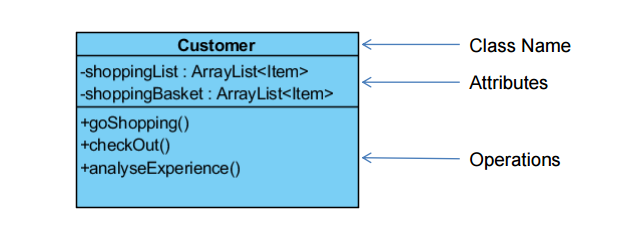
\includegraphics[scale = 0.6]{class1} %first class diagram

\newpage
Class diagrams are good because they provide a simple summary of the classes and relationships. But for larger projects, they can be a pain in the arse. Here's a reminder for the relationships (they don't give this on the slides so you can thank me later or by me a drink).
\\\\\\ % spacing for presentation reasons
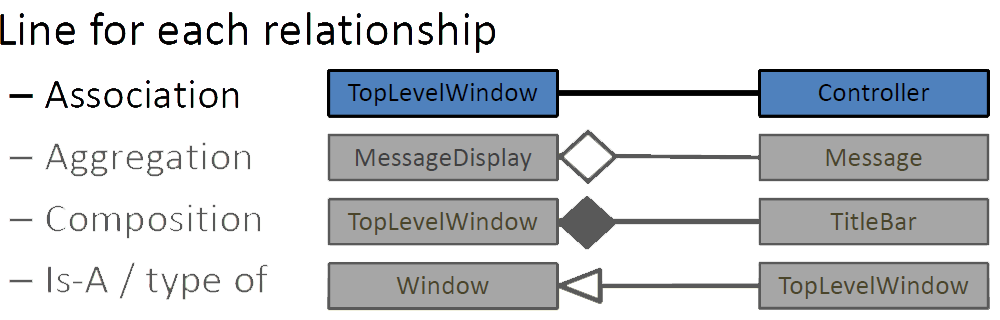
\includegraphics[scale = 0.35]{classRelationships}

The speak a bit about how important testing is. They express the importance of testing. As for types of testing, they can be broken down into:

\subsection{Testing Introduced}

\begin{itemize}
    \item \textbf{Regression Testing} $\longrightarrow$ This is when after you do a bug fix or change, you re-test to make sure that all of the old functionality is still there, and that the bug is fixed
    \item \textbf{Unit Testing} $\longrightarrow$ Automated tests to test the internal workings of the methods. The test is usually made to be small and as isolated as possible and so usually doesn't rely on other resources in the software
\end{itemize}

\section{Lecture 2 - More Advanced Java Programming}

In this lecture they discuss the `Java Collections Framework' and link it to some OO concepts.

\subsection{Java Collections Framework}

The best way to think about JCF is as a library. It is a collection of classes and interfaces that implement commonly reusable collection data structures. This includes things like ArrayLists. The framework not only contains data structures, but also algorithms e.g searching and sorting. On the lecture they describe the framework as `Container objects that contain objects'. The interface layout for JCF is as follows:

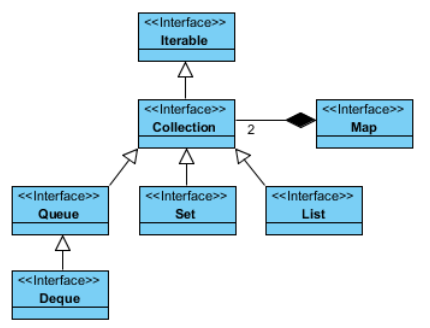
\includegraphics[scale = 0.8]{jcmLayout}

\begin{itemize}
    \item \textbf{Collection} $\longrightarrow$ Something that holds a dynamic collection of classes
    \item \textbf{Map} $\longrightarrow$ Defines mapping between keys and objects (two collections). The important thing to remember about the Map interface is that there are unique keys for each value. This interface is used in some data structures such as HashMaps, which will be explained later
    \item \textbf{Iterable} $\longrightarrow$ Basically a pointer to the collections content. You an move pointer to one of the objects within the collection for use
\end{itemize}

Most of these interfaces can be found in the java.util.* package, whilst the `Iterable' interface can be found in the java.lang.* package (probably don't need to know this). Here are some example implementations you may be familiar with:
\\\\
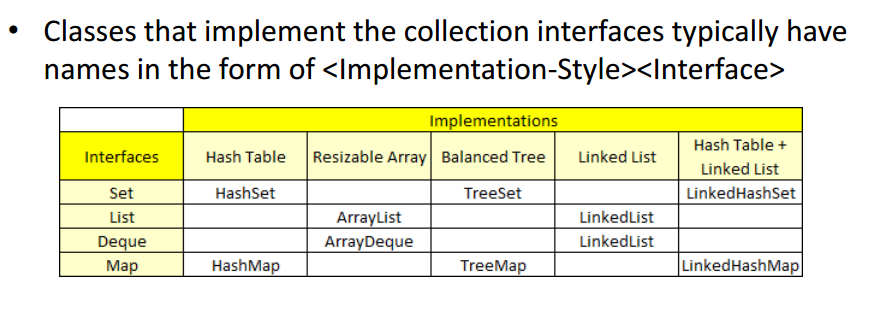
\includegraphics[scale = 0.65]{jcfImplementations}
\newpage

For the next part of the lecture they show code examples of the ArrayList, TreeSet and HashMap classes. ArrayLists are probably the most important so here's an example of that in use:

\begin{lstlisting}
import java.util.*;

public class ArrayListExample {
   public static void main(String args[]) {
      /*Creation of ArrayList: I'm going to add String
       *elements so I made it of string type */
	  ArrayList<String> obj = new ArrayList<String>();

	  /*This is how elements should be added to the array list*/
	  obj.add("Javascript is shit");
	  obj.add("Coffeescript is shit");
	  obj.add("Haskell is shit");
	  obj.add("Low level is best level");
	  obj.add("Pedro noob");

	  /* Displaying array list elements */
	  System.out.println("Currently the array list has following elements:"+obj);

	  /*Add element at the given index*/
	  obj.add(0, "U wot m8");
	  obj.add(1, "sowwy m8");

	  /*Remove elements from array list like this*/
	  obj.remove("Pedro noob");
	  obj.remove("Haskell is shit");

	  System.out.println("Current array list is:"+obj);

	  /*Remove element from the given index*/
	  obj.remove(1);

	  System.out.println("Current array list is:"+obj);
   }
}
\end{lstlisting}

Note that in the ArrayList declaration you have to give the type. This is because Java is too shit to understand it if you try to use a constructor instead.


\end{document}
